\lecture{12}{5 Dec. 14:20}{}

有一種等價的表達 NP 的方法,就是驗證器 (verifier) 的方法。

\begin{definition}
    A decision problem $L$ is in NP if there exists a polynomial-time algorithm $V$ such that for every instance $x$, \[
        x \in L \iff \exists\ c, |c| \leq |x|^{O(1)} \text{ such that } V(x, c) = \text{YES}
    \]
    Here, $c$ is called a certificate (or witness) for the instance $x$.
\end{definition}

\section{NP-Hard and NP-Complete}

\begin{definition}[NP-Hard]
    A problem $H$ is NP-Hard if for every problem $L$ in NP, there is a polynomial-time reduction from $L$ to $H$.
    \[
        \forall L \in \text{NP},\ L \leq_p H
    \]
    or equivalently, they are at least as hard as the all problems in NP.
\end{definition}

\begin{definition}[NP-Complete]
    A problem $C$ is NP-Complete if
    \begin{enumerate}
        \item $C$ is in NP, and
        \item $C$ is NP-Hard.
    \end{enumerate}
\end{definition}

NP-Complete 就是 NP 裡面最難的問題,如果我們能找到一個多項式時間的演算法來解決 NP-Complete 問題,那麼所有 NP 的問題都可以在 polynomial time 內解決,也就是說 NP = P。

\section{The question of P vs NP}

\begin{exercise}[Satisfiability (SAT) Problem]
    Given 
    \begin{itemize}
        \item \textbf{Input:} A Boolean formula $\phi$ in CNF (conjunctive normal form).
        \item \textbf{Output:} Is there a truth assignment to the variables that makes $\phi$ true?
    \end{itemize} 
\end{exercise}

\begin{theorem}[Cook-Levin Theorem]
    The Boolean satisfiability problem (SAT) is NP-Complete.
\end{theorem}

緊接著 Richard Karp 在 1972 年提出了 21 個 NP-Complete 問題,並且證明這些問題都是 NP-Complete 的,採用的是 polynomial-time reduction to SAT

\begin{figure}[H]
    \centering
    \includegraphics[width=0.8\textwidth]{Figures/complete.png}
    \caption{All NP-Complete Problems in Karp's 21 NP-Complete Problems}
\end{figure}

\section{Reduction}

\begin{prev}
    Problem A can be reduced (in polynomial time) to Problem B if the following condition holds: if problem B has a polynomial-time algorithm, then so does problem A. which is denoted as \[
        A \leq_p B
    \]
\end{prev}

\subsection{Hamiltonian Cycle Problem}

\begin{exercise}[Hamiltonian Cycle Problem]
    Given 
    \begin{itemize}
        \item \textbf{Input:} An undirected graph $G = (V, E)$.
        \item \textbf{Output:} Is there a simple cycle in $G$ that visits every vertex exactly once, i.e. contains all vertices in $V$.
    \end{itemize}
\end{exercise}

\begin{note}
    這並不是 Euler's tour,因為 Hamiltonian cycle 只需要經過每個點一次,而 Euler's tour 則是需要經過每條邊一次。
\end{note}

\begin{exercise}[Hamiltonian Path Problem]
    Given 
    \begin{itemize}
        \item \textbf{Input:} An undirected graph $G = (V, E)$ and two vertices $s, t \in V$.
        \item \textbf{Output:} Whether there is a simple path in $G$ from $s$ to $t$ that visits every vertex exactly once, i.e. contains all vertices in $V$.
    \end{itemize}
\end{exercise}

\newpage

我們可以將 Hamiltonian Cycle Problem reduce 到 Hamiltonian Path Problem,

\begin{corollary}
    Hamiltonian Cycle Problem $\leq_p$ Hamiltonian Path Problem.
\end{corollary}
\begin{proof}
    Let $G = (V, E)$ be an instance of Hamiltonian Cycle Problem. Suppose there is an polynomial-time algorithm $B$ for Hamiltonian Path Problem.
    We can get an new algorithm $A$ for Hamiltonian Cycle Problem as follows: \\

    Algorithm $A(G)$:
    \begin{quotation}
        We run $B(G, s, t)$ for each edge $st \in E(G)$. If all iteration return NO instance, then return NO; otherwise return YES.
    \end{quotation}
    \begin{note}
        我們必須確認三件事情
        \begin{enumerate}[label=$\arabic*^\circ$]
            \item $G$ 有一個包含所有頂點的 Hamiltonian cycle $A(G)$ 是否 return YES?
            \item $G$ 沒有包含所有頂點的 Hamiltonian cycle $A(G)$ 是否 return NO?
            \item Algorithm $A$ 是否在 polynomial time 內完成?
        \end{enumerate}
    \end{note}
    \begin{enumerate}[label=$\arabic*^\circ$]
        \item 如果 $G$ 有一個包含所有頂點的 Hamiltonian cycle,則對於 cycle 上的任意一條邊 $st$,將 $st$ 移除後,剩下的路徑就是一個從 $s$ 到 $t$ 的 Hamiltonian path。因此,當我們執行 $B(G, s, t)$ 時,會回傳 YES,進而使得 $A(G)$ 回傳 YES。
        \item 如果 $G$ 沒有包含所有頂點的 Hamiltonian cycle,則對於任意一條邊 $st$,將 $st$ 移除後,剩下的路徑不可能是從 $s$ 到 $t$ 的 Hamiltonian path。因此,當我們執行 $B(G, s, t)$ 時,會回傳 NO,進而使得 $A(G)$ 回傳 NO。
        \item Algorithm $A$ 需要對每一條邊執行一次 $B(G, s, t)$。假設圖 $G$ 有 $m$ 條邊,而算法 $B$ 在 polynomial time 內完成,即存在一個多項式函數 $p(n)$ 使得對於圖中有 $n$ 個頂點的情況下,算法 $B$ 的運行時間為 $O(n)^{O(1)}$。因此,算法 $A$ 的總運行時間為 $O(m \cdot \text{poly}(n))$。由於在一般情況下,邊數 $m$ 至多為 $\frac{n(n-1)}{2}$,因此總運行時間仍然是 polynomial time。
    \end{enumerate}
    Proof complete.
\end{proof}

\begin{vspace}{1em}

因為 Hamiltonian Cycle Problem 是 NP-Complete 的 (Karp's 21 NP-Complete Problems 之一),所以 Hamiltonian Path Problem 也是 NP-Complete 的(我們把 Hamiltonian Cycle Problem reduce 到 Hamiltonian Path Problem)。

\begin{exercise}[Longest Path Problem]
    Given
    \begin{itemize}
        \item \textbf{Input:} A graph $G$ and two vertices $u, v \in V(G)$.
        \item \textbf{Output:} a longest simple $uv$-path in $G$.
    \end{itemize}
\end{exercise}

\begin{vspace}{1em}

這是一個 NP 問題,可以找一個 NP verifier,只要這個 verifier 是 longest path,我就可以在 polynomial time 內驗證這個 path 是否是 longest path。

\newpage

\begin{corollary}
    Hamiltonian Path Problem $\leq_p$ Longest Path Problem.
\end{corollary}
\begin{proof}
    Let $(G, u, v)$ be an instance of Hamiltonian Path Problem. Suppose there is a polynomial-time algorithm $B$ for Longest Path Problem. We can get a new algorithm $A$ for Hamiltonian Path Problem as follows: \\

    Algorithm $A(G, u, v)$:
    \begin{quotation}
        We run $B(G, u, v)$ to get a longest simple $uv$-path $P$ of $G$. If $P$ passes through all vertices of $G$, then return YES; otherwise return NO.
    \end{quotation}
    \begin{enumerate}[label=$\arabic*^\circ$]
        \item 如果 $G$ 有一個包含所有頂點的 Hamiltonian path,則當我們執行 $B(G, u, v)$ 時,longest simple $uv$-path $P$ 必定包含所有頂點,$A(G, u, v)$ 回傳 YES。
        \item 如果 $G$ 沒有包含所有頂點的 Hamiltonian path,則當我們執行 $B(G, u, v)$ 時,回傳的 longest simple $uv$-path $P$ 不可能包含所有頂點,因此 $A(G, u, v)$ 回傳 NO。
        \item Algorithm $A$ 只需要執行一次 $B(G, u, v)$,假設圖 $G$ 有 $n$ 個頂點,而算法 $B$ 在 polynomial time 內完成,即存在一個多項式函數 $p(n)$ 使得對於圖中有 $n$ 個頂點的情況下,算法 $B$ 的運行時間為 $O(n)^{O(1)}$。因此,算法 $A$ 的總運行時間為 $O(\text{poly}(n))$,仍然是 polynomial time。
    \end{enumerate}
    Proof complete.
\end{proof}

\vspace{1em}

\subsection{Vertex Cover Problem}

\begin{exercise}[Vertex Cover Problem]
    Given
    \begin{itemize}
        \item \textbf{Input:} A graph $G = (V, E)$ and an integer $k$.
        \item \textbf{Output:} Determine whether $G$ admits a set of at most $k$ vertices that cover all edges in $E(G)$.
    \end{itemize}
\end{exercise}

\begin{exercise}[Independent Set Problem]
    Given
    \begin{itemize}
        \item \textbf{Input:} A graph $G = (V, E)$ and an integer $k$.
        \item \textbf{Output:} Determine whether $G$ contains a subset $S$ of $V(G)$ with $|S| \geq k$ such that two vertices in $S$ are not adjacent in $G$.
    \end{itemize}
\end{exercise}

\vspace{1em}

我們可以將 Vertex Cover Problem reduce 到 Independent Set Problem,藉由下面的觀察:

\newpage

\begin{corollary}
    Vertex Cover Problem $\leq_p$ Independent Set Problem and vice versa.
\end{corollary}
\begin{proof}
    Fir we claim that 
    \begin{claim}
        For each subset $S \subseteq V(G)$, $S$ is a vertex cover of $G$ if and only if $V(G) \setminus S$ is an independent set of $G$.
    \end{claim}
    \vspace{-1em}
    \begin{tmpexplanation}
        We proof the claim as follows:
        \begin{itemize}
            \item[``$\Rightarrow$''] 對於 $S$ 每個 $uv \in E(G)$ 都至少有一個端點在 $S$ 中。假設 $V(G) \setminus S$ 不是 independent set,則存在 $x, y \in V(G) \setminus S$ 使得 $xy \in E(G \setminus S)$,但 $xy$ 的兩個端點都不在 $S$ 中,與 $S$ 是 vertex cover 矛盾。
            \item[``$\Leftarrow$''] 對於 $V(G) \setminus S$ 中任意兩個頂點 $x, y$,$xy \notin E(G)$。假設 $S$ 不是 vertex cover,則存在 $uv \in E(G \setminus S)$,使得 $u, v \in V(G) \setminus S$,與 $V(G) \setminus S$ 是 independent set 矛盾。
        \end{itemize}
    \end{tmpexplanation}

    Let $(G, k)$ be an instance of Independent Set Problem. Suppose there is a polynomial-time algorithm $B$ for Vertex Cover Problem. We can get a new algorithm $A$ for Independent Set Problem as follows: \\

    Algorithm $A(G, k)$:
    \begin{quotation}
        We run $B(G, |V(G)| - k)$. If $B$ returns YES, then return YES; otherwise return NO.
    \end{quotation}
    \begin{enumerate}[label=$\arabic*^\circ$]
        \item By the claim, they are equivalent.
        \item Algorithm $A$ only needs to execute once $B(G, |V(G)| - k)$, and since $B$ runs in polynomial time, so does $A$.
    \end{enumerate}
    Proof complete.
\end{proof}

\subsection{3-SAT Problem}

\begin{definition*}
    Here is the definition of some variants of Satisfiability Problem, suppose $x$ is a Boolean formula in CNF.
    \begin{definition}[literal]
        A literal is either a variable $x_i$ or its negation $\neg x_i$ or we denote as $\overline{x_i}$.
    \end{definition}
    \begin{definition}[clause]
        If $x_1$, $x_2$, \ldots, $x_k$ are literals, then 
        \[
            x_1 \lor x_2 \lor \cdots \lor x_k
        \]
        is a clause.
    \end{definition}
    \begin{definition}[CNF formula]
        If $C_1$, $C_2$, \ldots, $C_m$ are clauses, then
        \[
            C_1 \land C_2 \land \cdots \land C_m
        \]
        is a CNF (Conjunctive Normal Form) formula.
    \end{definition}
    \begin{definition}[k-CNF formula]
        A $k$-CNF is a CNF each of whose clauses has $k$ literals.
    \end{definition}
\end{definition*}

\newpage

\begin{exercise}[3-SAT Problem]
    Given
    \begin{itemize}
        \item \textbf{Input:} A $k$-CNF $\phi$.
        \item \textbf{Output:} Determine whether $\phi$ is satisfiable.
    \end{itemize}
\end{exercise}

\begin{definition}
    Given a 3-CNF $\phi$, for each clause \[
        C_i = \alpha \lor \beta \lor \gamma
    \]
    we construct a triangle with vertices labeled $\alpha$, $\beta$, and $\gamma$. For any two vertices $x$ and $\overline{x}$ of the same variable $x$ that are complement to each other, we add an edge $x\overline{x}$ between them. The resulting graph is denoted as $G(\phi)$.
\end{definition}

\begin{theorem}
    The 3-CNF $\phi$ is satisfiable if and only if the graph $G(\phi)$ has an independent set of size $n$.
\end{theorem}
\begin{proof}
    We proof the theorem as follows:
    \begin{itemize}
        \item[``$\Rightarrow$''] If a truth assignment $T$ satisfies $\phi$, then $T$ satisfy at least one literal in each clause. We choose an arbitrary one statisfied literal from each clause(triangle). Since no two chosen literals are adjacent in $G(\phi)$, the set of chosen literals forms an independent set of size $n$ in $G(\phi)$.
        \item[``$\Leftarrow$''] Let $S$ be an independent set of size $n$ in $G(\phi)$. Each triangle in $G(\phi)$ contributes exactly one vertex to $S$. For each $\alpha \in S$, we assign $T(\alpha) = \text{true}$ and $T(\overline{\alpha}) = \text{false}$. Since no two vertices in $S$ are adjacent, this assignment is consistent. Moreover, since $S$ contains one vertex from each triangle, $T$ satisfies at least one literal in each clause of $\phi$. Therefore, $T$ is a satisfying assignment for $\phi$.
    \end{itemize}
    Proof complete.
\end{proof}

\begin{figure}[H]
    \centering
    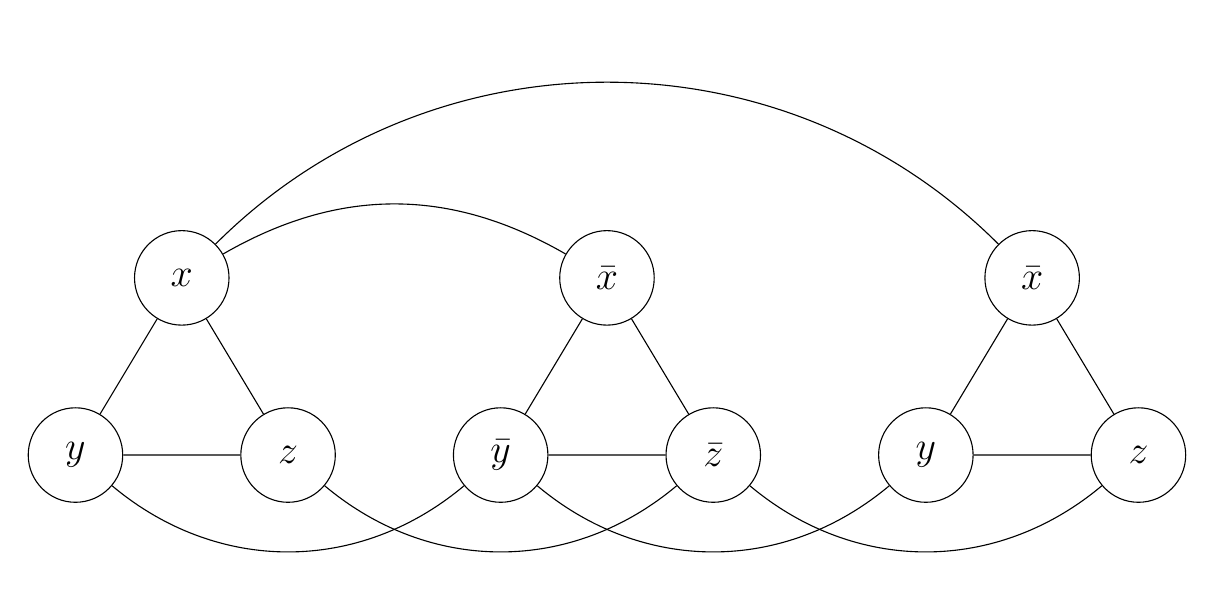
\begin{tikzpicture}[
        % 定義節點樣式:黑框、白底、圓形 (Automata 形式)
        node distance=1.5cm,
        state/.style={
            circle,
            draw=black,       % 黑色邊框
            inner sep=0pt,
            minimum size=1.2cm, % 節點大小
            font=\Large       % 字體大小
        },
        % 定義連線樣式
        thickedge/.style={
            black
        },
        scale=0.9
    ]
        % --- 1. 定義三個三角形 (Clauses) 的節點 ---
        
        % 第一個三角形 (Left)
        \node[state] (x1) at (0, 2.5) {$x$};
        \node[state] (y1) at (-1.5, 0) {$y$};
        \node[state] (z1) at (1.5, 0) {$z$};

        % 第二個三角形 (Middle)
        \node[state] (nx2) at (6, 2.5) {$\bar{x}$};
        \node[state] (ny2) at (4.5, 0) {$\bar{y}$};
        \node[state] (nz2) at (7.5, 0) {$\bar{z}$};

        % 第三個三角形 (Right)
        \node[state] (nx3) at (12, 2.5) {$\bar{x}$};
        \node[state] (y3) at (10.5, 0) {$y$};
        \node[state] (z3) at (13.5, 0) {$z$};

        % --- 2. 畫三角形內部的邊 (Clause Edges) ---
        \draw[thickedge] (x1) -- (y1) -- (z1) -- (x1);
        \draw[thickedge] (nx2) -- (ny2) -- (nz2) -- (nx2);
        \draw[thickedge] (nx3) -- (y3) -- (z3) -- (nx3);

        % --- 3. 畫衝突邊 (Conflict Edges - Curved Lines) ---
        
        % x 與 bar-x 的連接 (上方弧線)
        % x1 連到 nx2
        \draw[thickedge] (x1) edge[bend left=30] (nx2);
        % x1 連到 nx3 (跨度較大,弧度調高)
        \draw[thickedge] (x1) edge[bend left=45] (nx3);

        % y 與 bar-y 的連接 (下方弧線)
        % y1 連到 ny2
        \draw[thickedge] (y1) edge[bend right=40] (ny2);
        % ny2 連到 y3
        \draw[thickedge] (ny2) edge[bend right=40] (y3);

        % z 與 bar-z 的連接 (下方弧線)
        % z1 連到 nz2
        \draw[thickedge] (z1) edge[bend right=40] (nz2);
        % nz2 連到 z3
        \draw[thickedge] (nz2) edge[bend right=40] (z3);

    \end{tikzpicture}
    \caption{An example of constructing $G(\phi)$ from \\ $\phi = (x \lor y \lor z) \land (\bar{x} \lor \bar{y} \lor \bar{z}) \land (\bar{x} \lor y \lor z)$}
\end{figure}

\begin{corollary}
    3-SAT Problem $\leq_p$ Independent Set Problem.
\end{corollary}
\begin{proof}
    Let $\phi$ be an instance of 3-SAT Problem. Suppose there is a polynomial-time algorithm $B$ for Independent Set Problem. We can get a new algorithm $A$ for 3-SAT Problem as follows: \\

    Algorithm $A(\phi)$:
    \begin{quotation}
        Let $m$ be the number of clauses in $\phi$. Obtain the graph $G(\phi)$. We run $B(G(\phi), m)$. If $B$ returns YES, then return YES; otherwise return NO.
    \end{quotation}

    \begin{enumerate}[label=$\arabic*^\circ$]
        \item By the theorem, they are equivalent.
        \item Constructing $G(\phi)$ from $\phi$ can be done in polynomial time, as it involves creating a triangle for each clause and adding edges between complementary literals. Algorithm $A$ only needs to execute once $B(G(\phi), m)$, and since $B$ runs in polynomial time, so does $A$.
    \end{enumerate}
    Proof complete.
\end{proof}